\documentclass[10pt]{beamer}

\usetheme{CambridgeUS}
\usepackage[english, russian]{babel}
\usepackage[utf8]{inputenc}
\usepackage{caption}
\usepackage{etoolbox}
\usepackage{multicol}
\usepackage{listings}
\usepackage{wasysym}
\usepackage{mathtools}
\DeclarePairedDelimiter\ceil{\lceil}{\rceil}
\DeclarePairedDelimiter\floor{\lfloor}{\rfloor}

\definecolor{mygreen}{rgb}{0,0.6,0}
\lstset{
  basicstyle=\ttfamily\footnotesize,        % the size of the fonts that are used for the code
  breaklines=true,                 % automatic line breaking only at whitespace
  captionpos=b,                    % sets the caption-position to bottom
  commentstyle=\color{mygreen},    % comment style
  keywordstyle=\color{blue},       % keyword style
  stringstyle=\color{red},     % string literal style
  showstringspaces=false,
  morekeywords={include, printf},
  texcl=true     %<---- added
}


\title[\href{https://goo.gl/NRgp8K}{https://goo.gl/NRgp8K} (Term 1)]{Декартово дерево}
\author[Гусев Илья, Булгаков Илья]{Гусев Илья, Булгаков Илья}
\institute[МФТИ] 
{Московский физико-технический институт\\*}
\date{Москва, 2018}
\subject{Computer Science}

\begin{document}

\begin{frame}
  \titlepage
\end{frame}

\begin{frame}{Содержание}
\tableofcontents
\end{frame}

\section{Проблемы бинарных деревьев поиска}
\begin{frame}[fragile]{Проблемы бинарных деревьев поиска}{Вырождение}
\begin{center}
    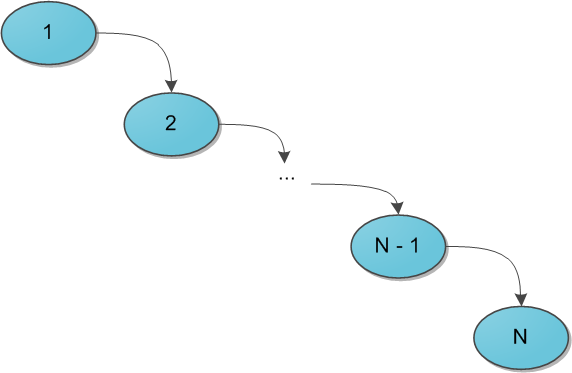
\includegraphics[width=8cm, height=5cm]{Term_1/Source/Pirctures/tree_problem.png}\\
    O(N) на вставку и удаление
\end{center}
\end{frame}

\begin{frame}[fragile]{Проблемы бинарных деревьев поиска}{Неодназначность}
\begin{center}
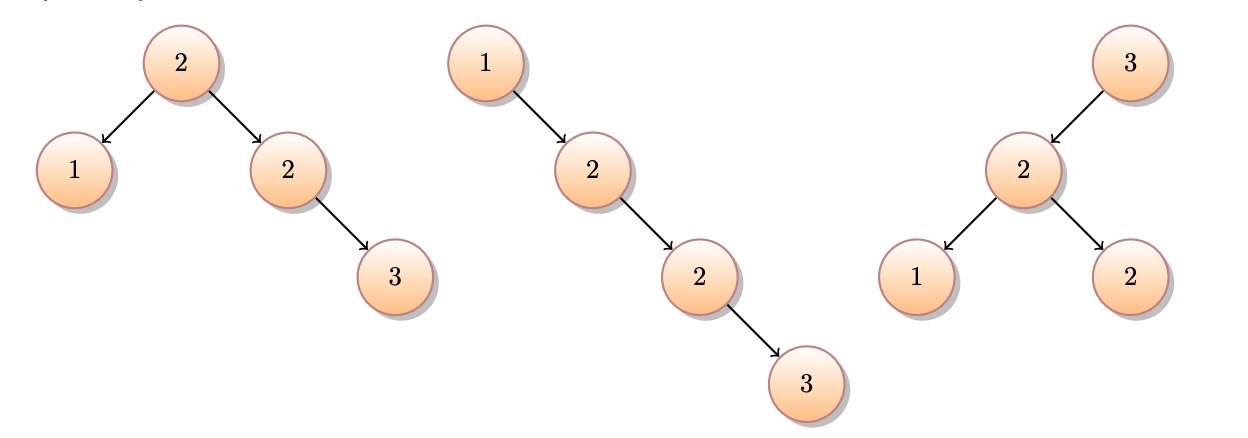
\includegraphics[width=12cm, height=4.3cm]{Term_1/Source/Pirctures/tree_ways.jpg}
\\
Зависит от порядка вставки элементов
\end{center}
\end{frame}

\section{Декартово дерево}
\subsection{Общее описание}
\begin{frame}[fragile]{Декартово дерево}{Общее описание}
\begin{itemize}
    \item Бинарное дерево поиска по ключу x
    \item Куча по приоритету y
    \item В одной вершине храним x и y
    \item Случайные приоритеты $\rightarrow$ балансировка
    \item Другие названия:
    \begin{enumerate}
        \item treap (tree + heap)
        \item дуча (дерево + куча)
        \item дерамида (дерево + пирамида)
        \item курево (куча + дерево)
    \end{enumerate}
\end{itemize}
\end{frame}

\subsection{Почему декартово?}
\begin{frame}[fragile]{Почему декартово?}
\begin{center}
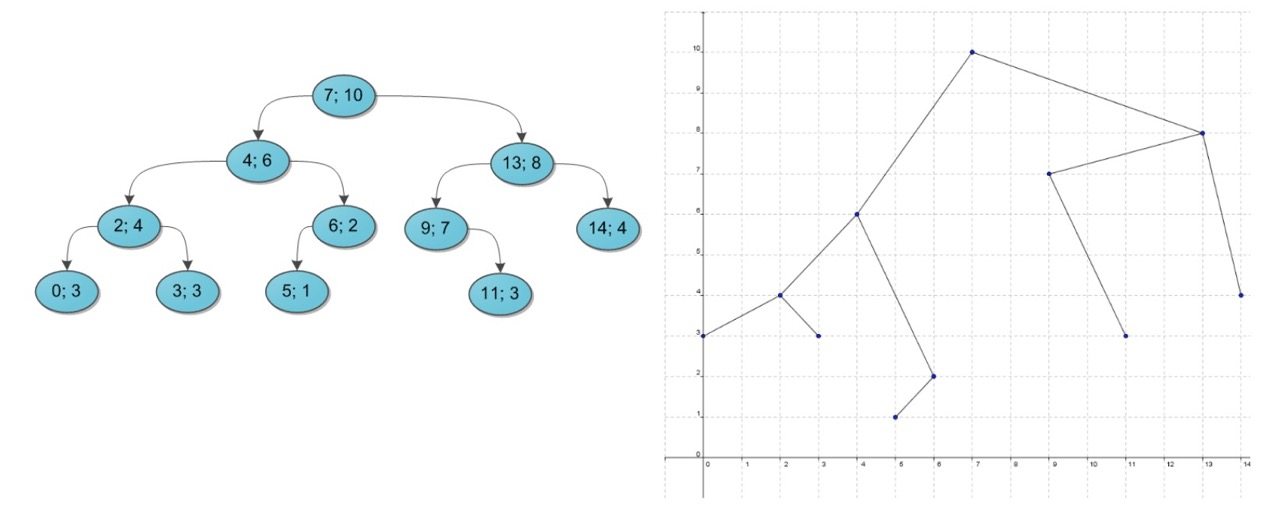
\includegraphics[width=12cm, height=5cm]{Term_1/Source/Pirctures/treap.jpg}
\\
По x - дерево поиска, по y - куча
\end{center}
\end{frame}

\subsection{Операции}
\begin{frame}[fragile]{Декартово дерево}{Внешние операции}
\begin{itemize}
    \item Вставка элемента: в среднем $O(log(N))$
    \item Удаление элемента: в среднем $O(log(N))$
    \item Поиск по ключу: в среднем $O(log(N))$
    \item Построение по отсортированному массиву за $O(n)$
    \item Поиск k-порядковой статистики: в среднем $O(log(N))$, нужно $O(n)$ доп. памяти
    \item Сумма, минимум, максимум на отрезке: в среднем $O(log(N))$, нужно $O(n)$ доп. памяти
\end{itemize}
\end{frame}

\begin{frame}[fragile]{Декартово дерево}{Внутрненние операции}
\begin{itemize}
    \item Merge - склейка 2 деревьев; все ключи одного меньше всех ключей другого: в среднем $O(log(N))$
    \item Split - разрезание по ключу на 2 дерева: в среднем $O(log(N))$
\end{itemize}
\end{frame}

\subsection{Merge}
\begin{frame}[fragile]{Декартово дерево}{Merge}
\begin{center}
    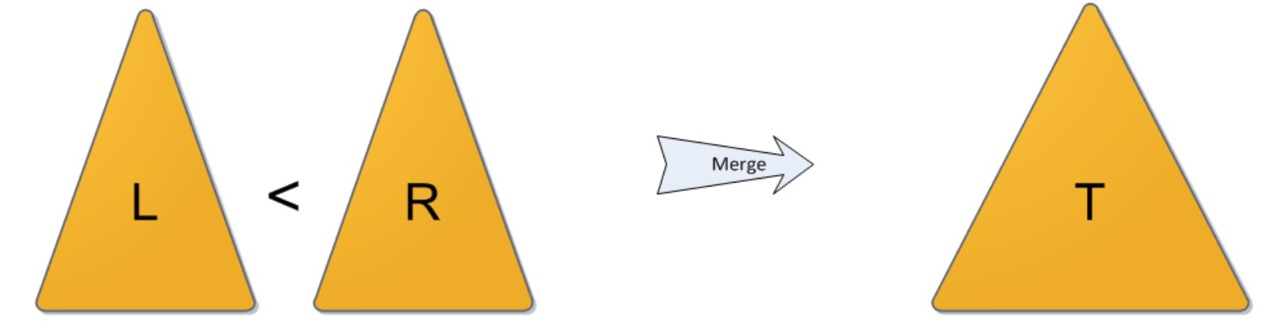
\includegraphics[width=12cm, height=3cm]{Term_1/Source/Pirctures/treap_merge.jpg}\\
\end{center}
\begin{itemize}
    \item Все ключи дерева L меньше ключей дерева R
    \item Б.о.о. приоритет (y) корня левого дерева больше приоритета корня правого дерева $\rightarrow$ новый корень - корень левого дерева
\end{itemize}
\end{frame}

\begin{frame}[fragile]{Декартово дерево}{Merge}
\begin{center}
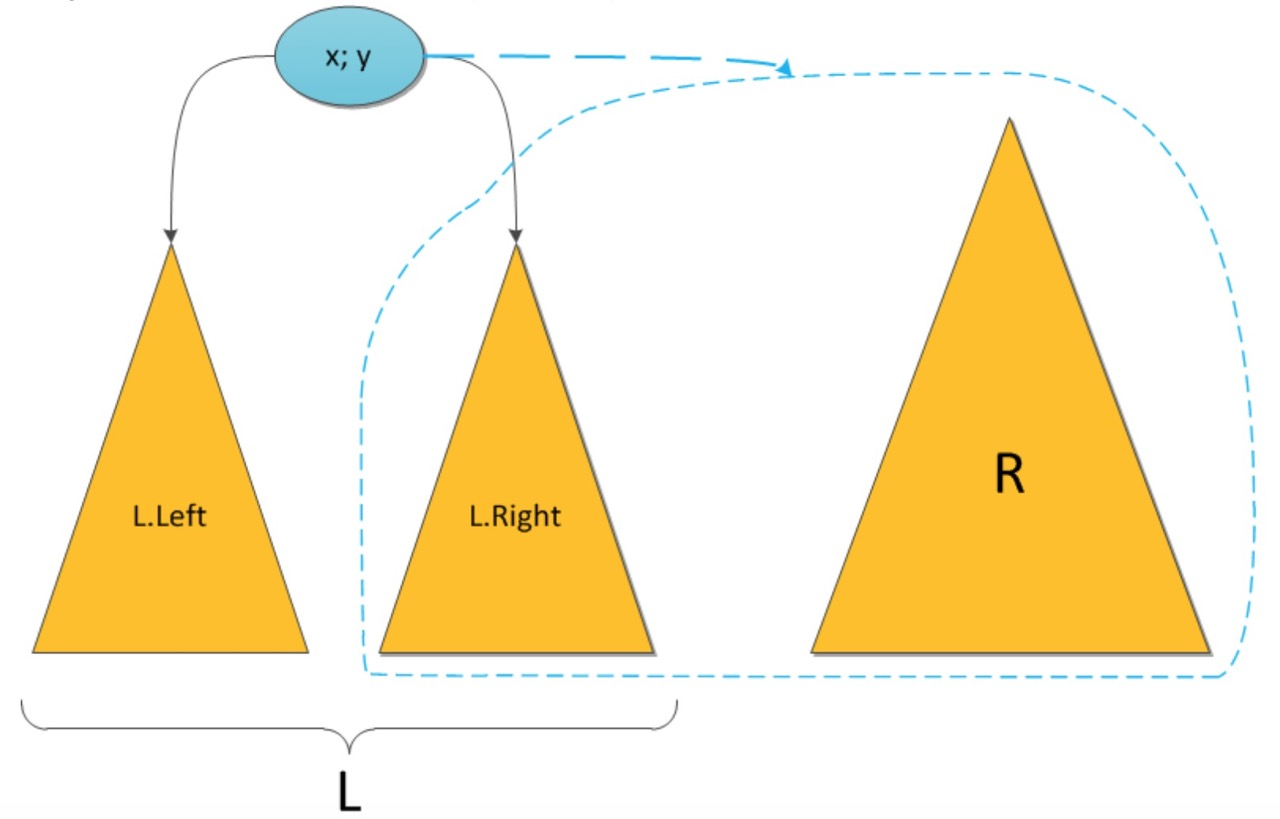
\includegraphics[width=8cm, height=4cm]{Term_1/Source/Pirctures/treap_merge_step.jpg}
\end{center}
\begin{itemize}
    \item Тогда R - точно в правом поддереве нового корня
    \item L.Left -  точно левое поддерво нового корня
    \item Рекурсивно сливаем L.Right и R
    \item База рекурсии: хотя бы одно дерево пустое
\end{itemize}
\end{frame}

\begin{frame}[fragile]{Декартово дерево}{Merge}
\begin{itemize}
    \item Сложность: сумма высот деревьев, в среднем $O(log(n) + log(m))$
\end{itemize}
\end{frame}

\subsection{Split}
\begin{frame}[fragile]{Декартово дерево}{Split}
\begin{center}
    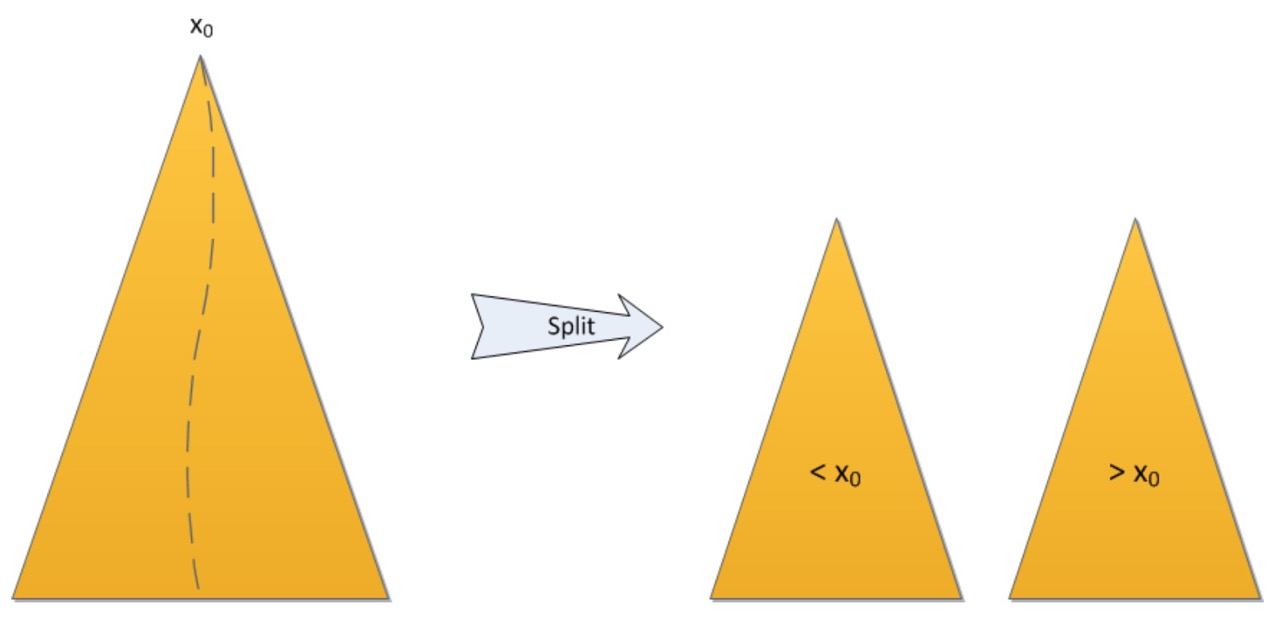
\includegraphics[width=10cm, height=4cm]{Term_1/Source/Pirctures/treap_split.jpg}\\
\end{center}
\begin{itemize}
    \item Разделяем по ключу $x_o$
    \item Б.о.о ключ корня меньше $x_0$
\end{itemize}
\end{frame}

\begin{frame}[fragile]{Декартово дерево}{Split}
\begin{center}
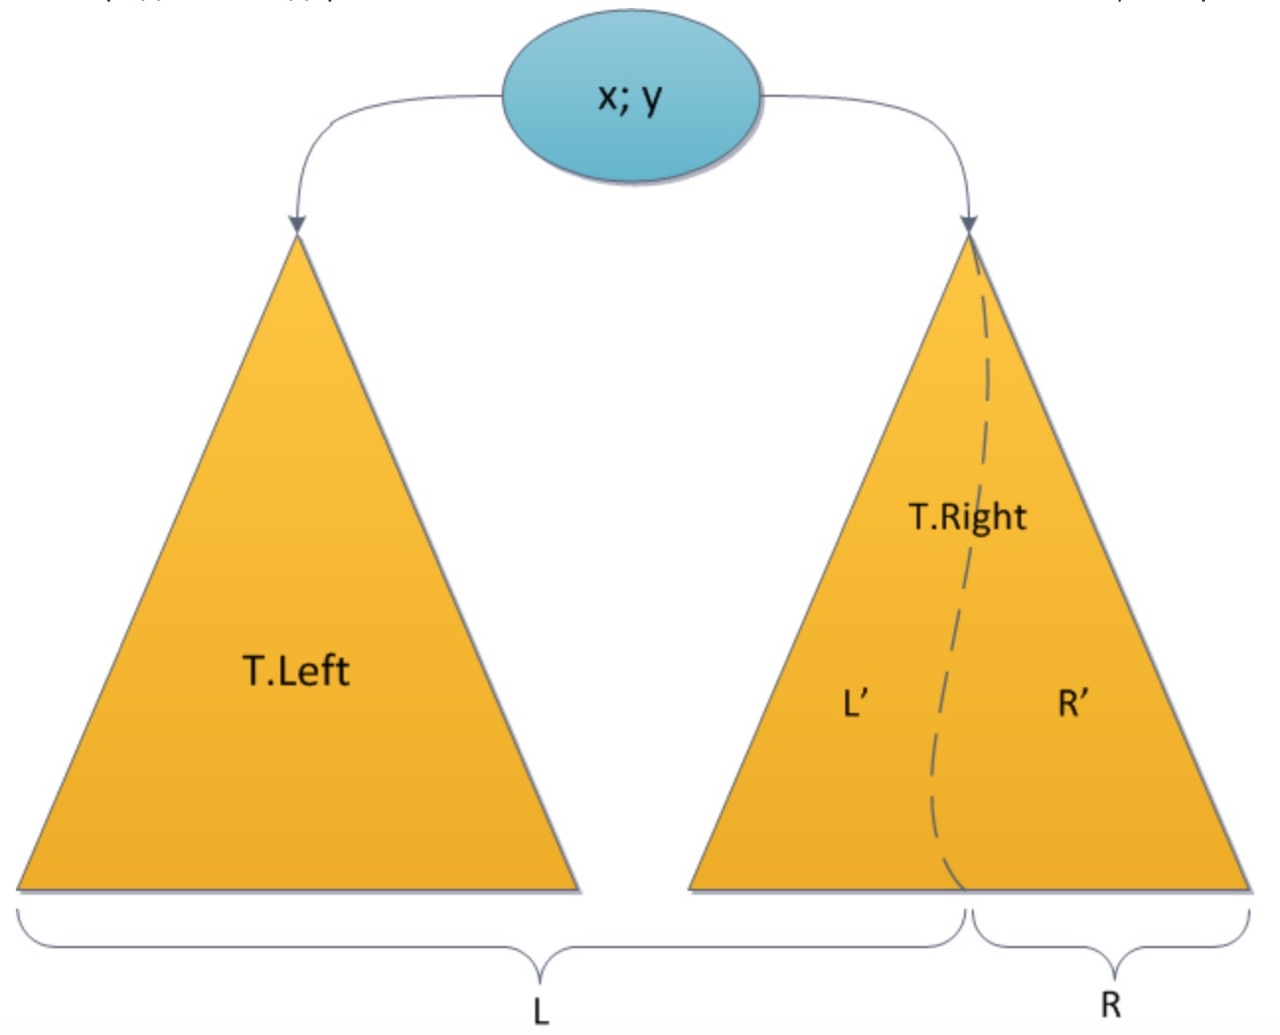
\includegraphics[width=6cm, height=4.5cm]{Term_1/Source/Pirctures/treap_split_step.jpg}
\end{center}
\begin{itemize}
    \item Рекурсивно делим правое поддерво корня на L' и R'
    \item L' - новое правое поддерво корня
\end{itemize}
\end{frame}

\begin{frame}[fragile]{Декартово дерево}{Split}
\begin{itemize}
    \item Сложность: высота изначального дерева, в среднем $O(log(n))$
\end{itemize}
\end{frame}

\subsection{Insert}
\begin{frame}[fragile]{Декартово дерево}{Insert}
\begin{center}
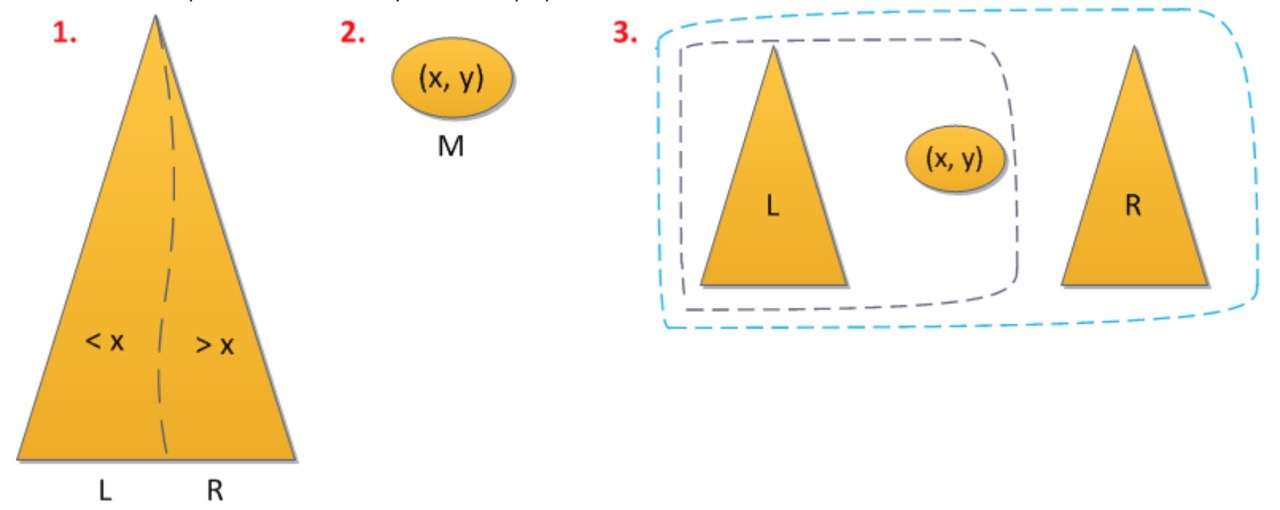
\includegraphics[width=12cm, height=4.5cm]{Term_1/Source/Pirctures/treap_insert.jpg}\\
Вставка элемента  (x, y)\\
1 Split + 2 Merge
\end{center}
\end{frame}

\subsection{Remove}
\begin{frame}[fragile]{Декартово дерево}{Remove}
\begin{center}
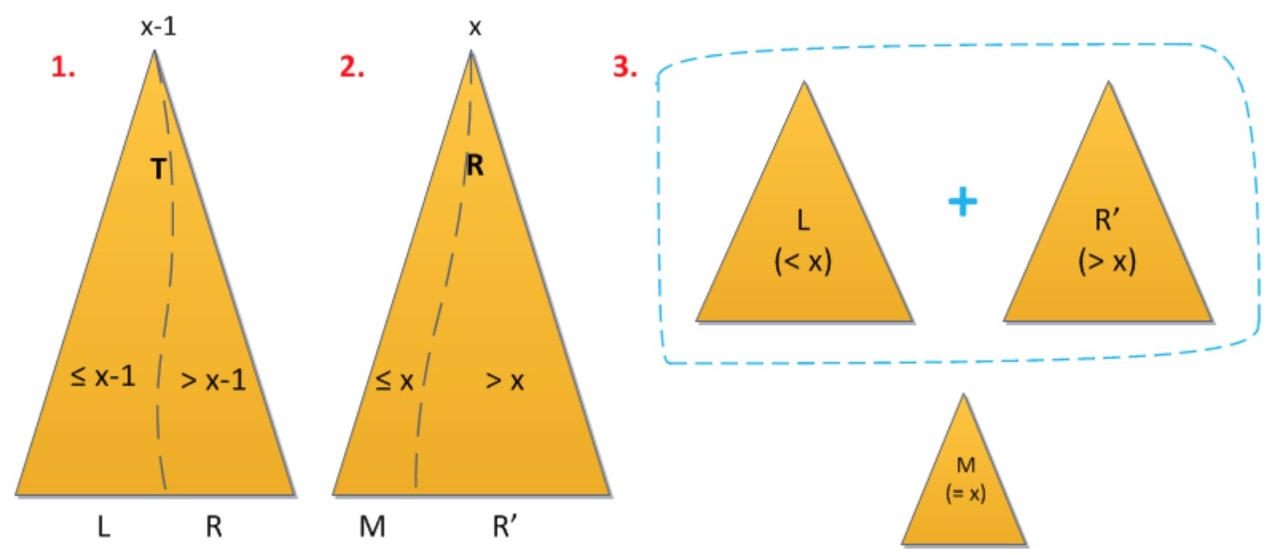
\includegraphics[width=12cm, height=4.5cm]{Term_1/Source/Pirctures/treap_remove.jpg}\\
Удаление элементов с ключом x\\
2 Split + 1 Merge
\end{center}
\end{frame}

\subsection{Build}
\begin{frame}[fragile]{Декартово дерево}{Build}
\begin{itemize}
    \item В случае неотсортированного массива - n вставок, $O(n\cdot log(n))$
    \item В случае отсортированного массива всегда рассматриваем самую правую ветку и вставляем в самую правую ветку $\rightarrow$ каждый элемент рассматривается не больше 2 раз $\rightarrow O(n)$ 
    \item Нужны ссылки на предков и на последнюю вставленную вершину
\end{itemize}
\end{frame}

\begin{frame}[fragile]{Декартово дерево}{Build-1}
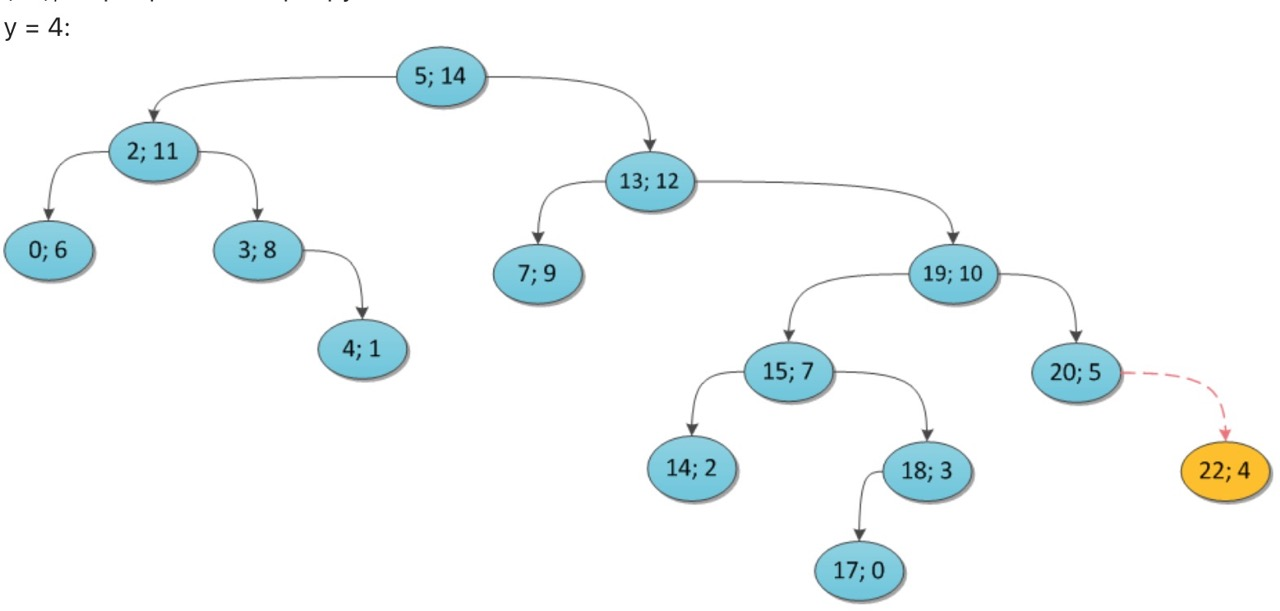
\includegraphics[width=12cm, height=6cm]{Term_1/Source/Pirctures/treap_insert_4.jpg}\\
\end{frame}

\begin{frame}[fragile]{Декартово дерево}{Build-2}
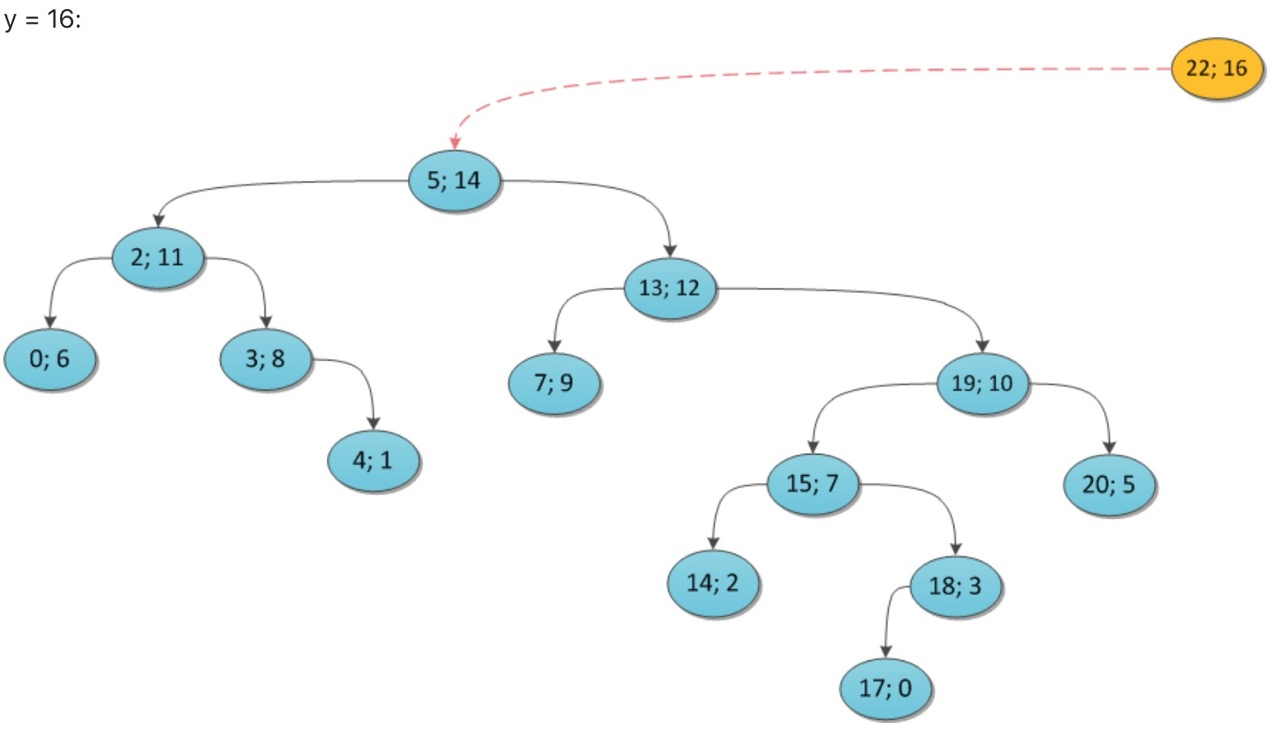
\includegraphics[width=12cm, height=6.5cm]{Term_1/Source/Pirctures/treap_insert_16.jpg}\\
\end{frame}

\begin{frame}[fragile]{Декартово дерево}{Build-3}
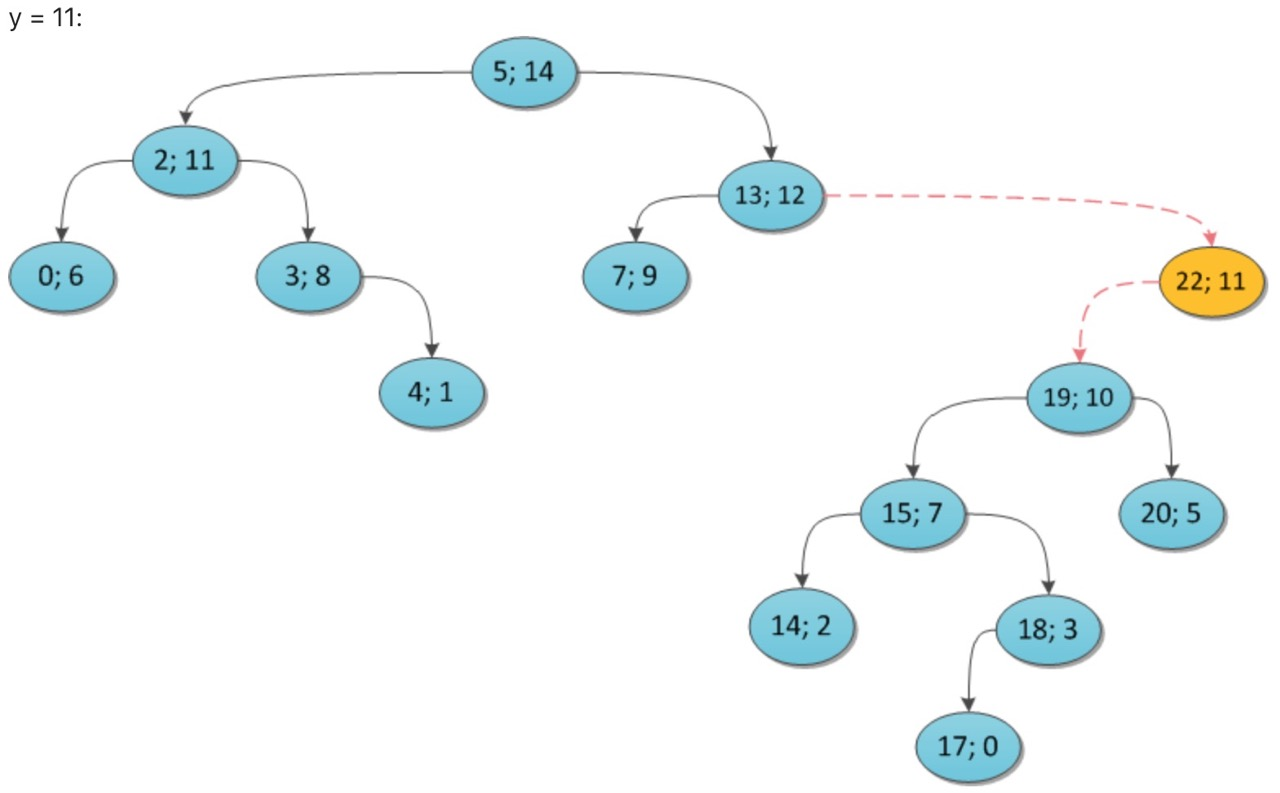
\includegraphics[width=12cm, height=7cm]{Term_1/Source/Pirctures/treap_insert_11.jpg}\\
\end{frame}

\subsection{K-ая порядковая статистика}
\begin{frame}[fragile]{K-ая порядковая статистика}
\begin{center}
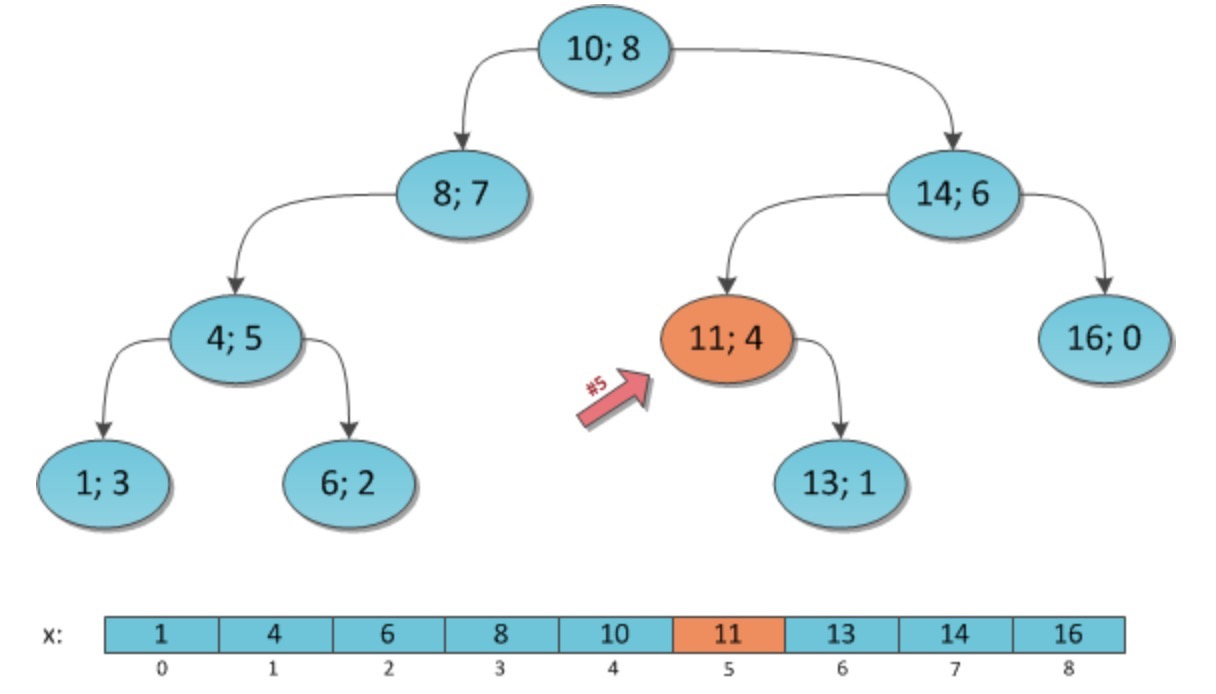
\includegraphics[width=10cm, height=6cm]{Term_1/Source/Pirctures/treap_naive_korder.jpg}\\
Используем обычный обход бинарного дерева поиска $\rightarrow O(n)$
\end{center}
\end{frame}

\begin{frame}[fragile]{K-ая порядковая статистика}{Через размер поддеревьев}
\begin{center}
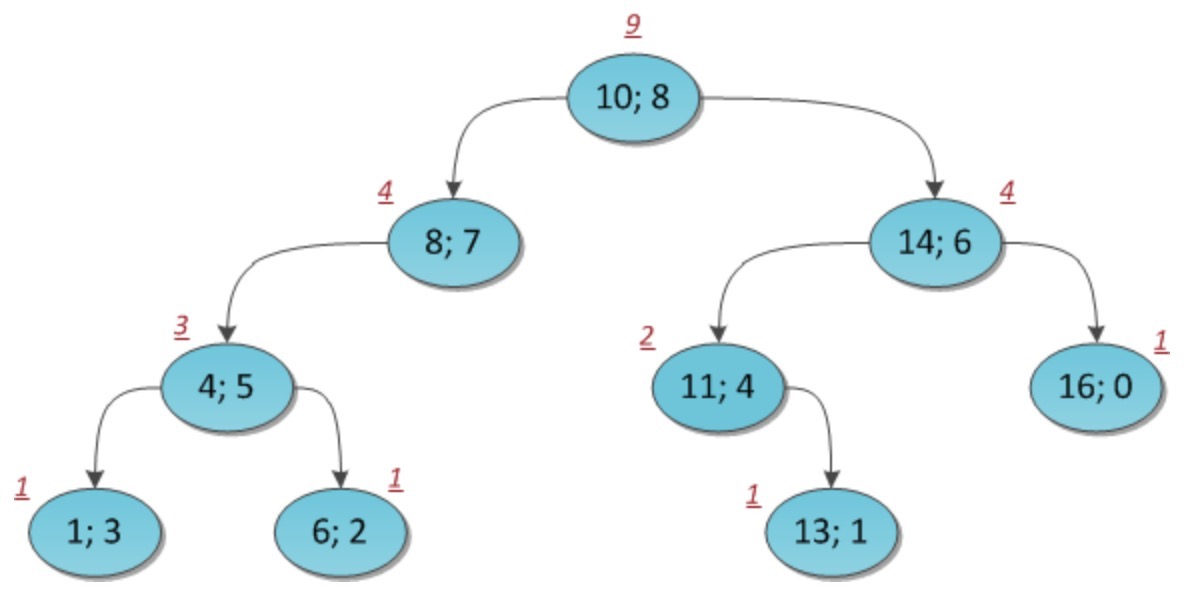
\includegraphics[width=7cm, height=4cm]{Term_1/Source/Pirctures/treap_subtrees.jpg}\\
\end{center}
\begin{itemize}
    \item Для каждой вершины храним размер её поддерева
    \item Спускаемся с корня
    \item Если размер левого поддерева равен K - мы победили
    \item Если размер левого поддерева больше K, спускаемя в него и повторяем
    \item Если размер левого поддерева меньше K, уменьшаем K и спускаемся в правое поддерево
\end{itemize}
\end{frame}

\begin{frame}[fragile]{K-ая порядковая статистика}{Через размер поддеревьев}
\begin{center}
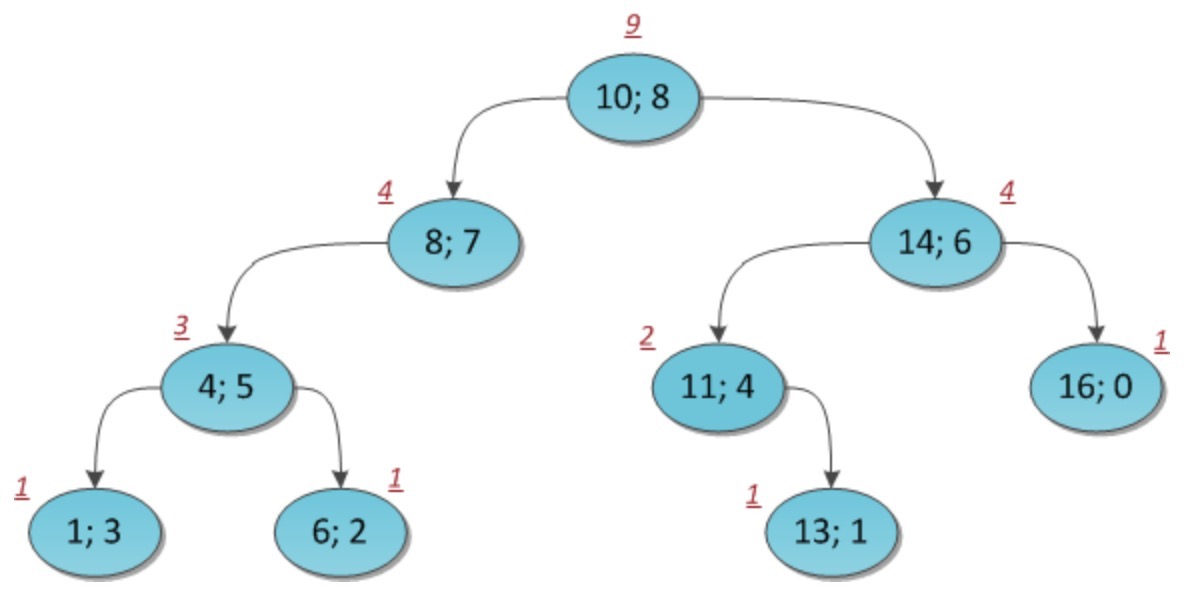
\includegraphics[width=7cm, height=4cm]{Term_1/Source/Pirctures/treap_subtrees.jpg}\\
\end{center}
\begin{itemize}
    \item Сложность: $O(log(n))$
    \item Но при вставке элементов нужно пересчитывать размеры, наивно: $O(n)$
    \item Модифицируем Merge и Split - плюс O(1) операций на каждый их шаг
    \item Не только размер поддеревьев, а любые значения: max, min, sum
\end{itemize}
\end{frame}

\subsection{Неявный ключ}
\begin{frame}[fragile]{Декартово дерево по неявному ключу}
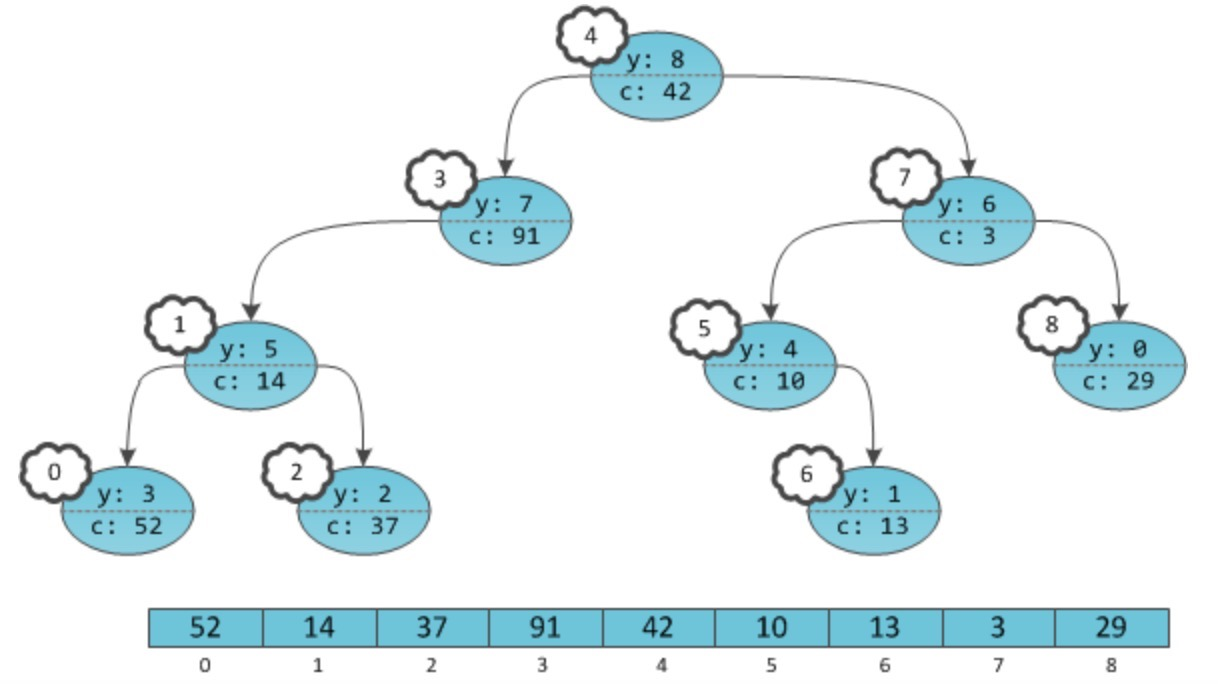
\includegraphics[width=9cm, height=5.5cm]{Term_1/Source/Pirctures/treap_implicit.jpg}\\
\begin{itemize}
    \item Рассматриваем дерево как массив, ключи - индексы в массиве
    \item Слияние 2 массивов, вставка элемента в произвольное место, удаление элемента из произвольного места и много другого: в среднем $O(log(n))$!
\end{itemize}
\end{frame}

\appendix
\section<presentation>*{\appendixname}
\subsection<presentation>*{Useful links}

\begin{frame}[allowframebreaks]
  \frametitle<presentation>{Полезные ссылки}
    
  \begin{thebibliography}{10}
{
  \beamertemplatearticlebibitems
  
  \bibitem{habr}
  \texttt{Цикл 'Декартово дерево' на Хабре}
  \newblock \href{https://habr.com/post/101818/}{\texttt{https://habr.com/post/101818/}}
  
  \bibitem{emaxx}
  \texttt{E-maxx: Декартово дерево (treap, дерамида)}
  \newblock \href{http://www.e-maxx-ru.1gb.ru/algo/treap}{\texttt{http://www.e-maxx-ru.1gb.ru/algo/treap}}
  
  \bibitem{zksh}
  \texttt{Конспкеты лекций ЗКШ: декартово дерево}
  \newblock \href{https://bit.ly/2ORjVU2}{\texttt{https://bit.ly/2ORjVU2}}
  
  \bibitem{zksh}
  \texttt{Викиконспекты: Декартово дерево}
  \newblock \href{https://bit.ly/2CcsxOa}{\texttt{https://bit.ly/2CcsxOa}}

}


  \end{thebibliography}
\end{frame}

\end{document}


